\chapter{Analysis}
\section{Direct Observables: Building Blocks of the Measurement}
\textbf{TO DO: ADD A FIGURE OF THE PHENIX COORDINATE SYSTEM}
\subsection{Central Arm Tracks}
This analysis use central arm tracks. A central arm track is a charged particle emitted from the heavy ion collision and detected by the PHENIX central arms.
There are 2 central arms and each one covers $\eta < |0.35|$ and $\frac{\pi}{2}$ in azimuth. The drift chamber provides momentum information and the
pad chambers provide track quality metrics. The RICH provides electron identification. 
The physics parameters of central arm tracks relevant to this analysis is the momentum vector: $p = (p_x, p_y, p_z)$. The momentum of CNT tracks is defined at the
collision vertex. CNT have good momentum resolution (\textbf{TO DO: QUANTIFY THIS}). In p+Au collisions, the average number of reconstructed CNT (before cuts) is (\textbf{TO DO: QUANTIFY THIS}).
\subsection{FVTX Clusters}
This analysis uses clusters from the forward vertex detector (FVTX). The FVTX detects charged particles traveling through its silicon layers. The intersection between the charged particle
and the FVTX detector is recorded in each of the 4 layers the particle goes through. Each intersection is known as a cluster. Each cluster is thought to be produced from a single charged particle. These clusters have a position resolution in x and y ( or r and $\phi$)
(\textbf{TO DO: QUANTIFY THIS}) and have a z resolution that is the width of the FVTX layer. The FVTX acceptance is $1 < | \eta | < 3$ and spans the full azimuth.
\subsection{BBC PMTs}
This analysis uses photomultipliers (PMTS) from the beam beam counter (BBC). The BBC detects charged particles traveling through its scintillator material. The BBC acceptance is $3.1 < |\eta| < 3.9$ and spans the full azimuth. The BBC provides position information in x, y, and z and, like the FVTX, the x and y ( or r and $\phi$) resolution differ from the z resolution in that the z resolution is simply the width of the active area of the BBC. In addition to position information, the BBC provides charge information which is calibrated to roughly correspond to the number of charged particles detected by each PMT per event.
%\section{Two-particles Correlation}
%\subsection{Measurement in p+p and p+Au}
\section{Event Plane Method}
The event plane method is a way of measuring the long range correlations in the spray of particles from a heavy ion collision. The event plane method works by calculating a mathematical object
from the data called an event plane. This event plane is defined for each flow harmonic and is sometimes denoted as $\Psi_n$. The definition for $\Psi_n$ is related to the calculation of the Q-vector:
\begin{align}
Q_x &= \sum( w_i * \cos(n * \phi_i)) \\
Q_y &= \sum( w_i * \sin(n * \phi_i)) \\
Q_w &= \sum( w_i ) \\
\Psi_n &= \arctan( \frac{Q_y}{Q_x} ).
\end{align}
The $Q_w$ component of the Q-vector is only used during the event plane calibration.
Once the event plane has been calculated, the flow harmonics ($v_n$) are calculated as
\begin{equation}
v_n = \frac{<<\cos(n(\phi - \Psi_n))>>}{Resolution(\Psi_n)},
\end{equation}
where $<<>>$ means averaged over each event and each $\phi$ value and the resolution of $\Psi_n$ is calculated using the 3-subevent method. It is important to note the the set of particles used to calculate $\Psi_n$ and $\phi$ must be different in order to avoid
autocorrelations. This is usually done by imposing an $\eta$ gap between to two particle sets.

For this analysis, the event plane is calculated separately for each of the forward detectors mentioned above, the BBC and the FVTX. For the FVTX, the Q-vector is calculated in each event as
\begin{align}
Q_x &= \sum^{NFVTXClus}_i( \cos(n * \phi_i)) \\
Q_y &= \sum^{NFVTXClus}_i( \sin(n * \phi_i)) \\
\phi_i &= \arctan(\frac{FVTXClus_{y}^i}{FVTXClus_{x}^i})
\end{align}
where NFVTXClus is the number FVTX clusters in that event and $FVTXClus_{y,x}^i$ are the $x$ and $y$ components of the $i$th FVTX Cluster in that event. This Q-vector is calculated with no cluster dependent weight factor as each cluster is taken to be equal weight (since no charge information is available in the FVTX).

For the BBC, the Q-vector is calculated in each event as
\begin{align}
Q_x &= \sum^{NPMT}_i( w_i \cos(n * \phi_i)) \\
Q_y &= \sum^{NPMT}_i( w_i \sin(n * \phi_i)) \\
Q_w &= \sum( w_i ) \\
\phi_i &= \arctan(\frac{PMT_{y}^i}{PMT_{x}^i}) 
\end{align}
where $w_i$ is the charge collected on the PMT and NPMT is the number of PMTs that fired (above threshold) in each event.

Finally, the $v_n$ are calculated using a combination of the BBC or FVTX Q-vectors and the CNT tracks as
\begin{equation}
v_n = \frac{\left<\left<\cos(n(\phi^{CNT} - \Psi^{BBC,FVTX}_n))\right>\right>}{Resolution(\Psi^{BBC,FVTX}_n)}.
\end{equation}
In this analysis, I will be exclusively focusing on the second harmonic $v_2$. The reason for this is two-fold:
\begin{enumerate}
	\item{The second harmonic is usually the largest and easiest to measure harmonic.}
	\item{The second harmonic is physically interesting because it is thought to correspond with flow. The first harmonic is thought to correspond momentum conservation.}
\end{enumerate}
\subsection{Event Plane Flattening Calibration}
In order for the event plane to be a useful in making a $v_n$ measurement, the event plane must be calibrated. For the event plane method, a physical assumption is made that the true
distribution of $\Psi_n$ angles will be uniform. In other words, there is no preferred event plane angle in heavy ion collisions; on average there should an equivalent amount of events where the
event plane is oriented at 0 radians and at $\frac{\pi}{2}$. So if the measured $\Psi_n$ distribution is not flat then it could come from a variety of sources such as variations in the efficiency of detecting charged particles as a function of $\phi$. Thus, the event plane calibration seeks to restore the $\Psi_n$ distribution to the physical expectation of uniformity.

The method used in this analysis to achieve this is a "re-centering" and "flattening" calibration. In order to better understand this calibration, it is useful to examine an example uncalibrated $\Psi_n$ distribution.
%\begin{figure}[htbp]
%\begin{center}
%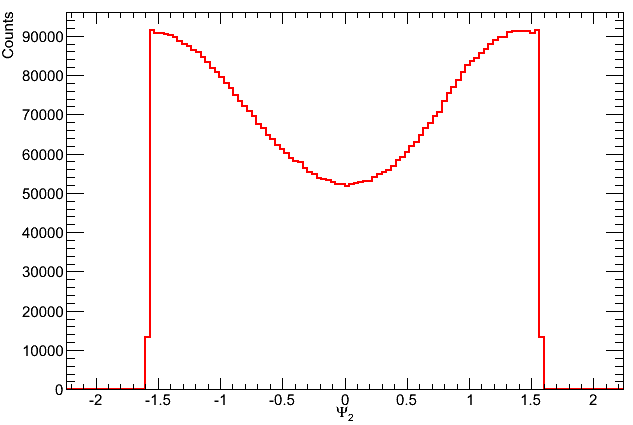
\includegraphics[width=0.65\linewidth]{figs/example_raw_psi2.png}
%\caption{This is the BBC-S $\Psi_2$ distribution before any calibration. The range of the $\Psi_2$ resolution is from $\frac{-\pi}{2}$ to $\frac{\pi}{2}$ because of the periodicity. 
%The raw distribution has a sinusoidal shape.}
%\end{center}
%\label{fig:raw_psi}
%\end{figure}
The red curve in Fig. ~\ref{fig:calibrated_psi} depicts a significant deviation from uniformity in the $\Psi_2$ distribution which would distort the $v_2$ measurement. 
A combination of effects cause there to be a depletion of $\Psi_2$ values at 0.0 radians and an enhancement at $\frac{\pi}{2}$ radians. The flattening calibration attempts to offset this 
lack of uniformity by systematically shifting each event's raw $\Psi_2$ value by an amount corresponding to the amount the $\Psi_2$ distribution is nonuniform. The more that the raw $\Psi_2$
distribution is nonuniform, the more significant that the flattening calibration must systematically shift each $\Psi_2$ value in order to restore uniformity. Thus, it is in the analyzer's best interest
to provide the flattest possible $\Psi_2$ distribution before performing the flattening calibration.
\begin{figure}[!h]
\begin{center}
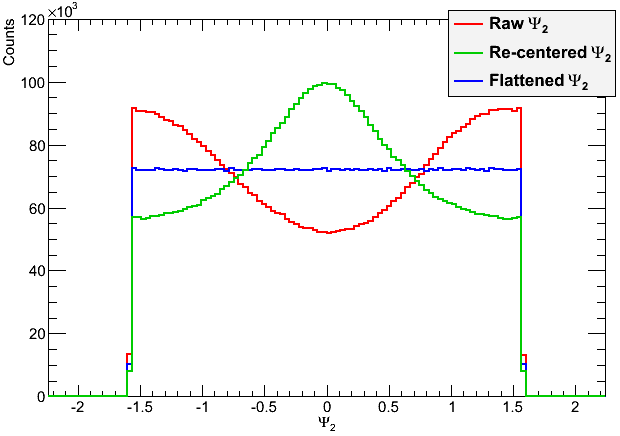
\includegraphics[width=0.65\linewidth]{figs/flattened_example.png}
\caption{This is the FVTX-S $\Psi_2$ distribution projected over all z-vertex bins at different steps during the calibration. The range of the $\Psi_2$ resolution is from -$\frac{\pi}{2}$ to $\frac{\pi}{2}$ because of the periodicity. 
The raw (in red) $\Psi_2$ distribution has a sinusoidal shape. The re-centered (in green) $\Psi_2$ distribution moves the peak to 0.0 radians and changes the width. The flattened (in blue) 
$\Psi_2$ distribution spread out the counts so that there is uniformity. Each calibration step preserves the integral.}
\end{center}
\label{fig:calibrated_psi}
\end{figure}

The flattening calibration requires two steps to completely flatten the $\Psi_n$ distribution. The first step of the calibration is to re-center the peak of the raw $\Psi_n$ distribution to be at 
0.0 radians and to resize the width of the peak. The second step is to Fourier transform the re-centered distribution and use the transformation to shift the $\Psi_n$ values to a uniform distribution. With flattening, each $\Psi_n$ is transformed to $\Psi_n + \Delta\Psi_n$ where $\Delta\Psi_n$ is defined as
\begin{equation}
\Delta\Psi_n = \sum^{N}_{i=1}\left(\frac{2}{i}\left(\sin(i \Psi)F^{\cos}_{i}(f(\Psi_n))-\cos(i \Psi)F^{\sin}_{i}(f(\Psi_n)\right)\right),
\label{eq:deltapsi}
\end{equation}
where $N$ is the number of components, $F^{\cos}_{i}(f(x))$ is the $i$th component of the cosine Fourier transform of $f(x)$, and $f(\Psi_n)$ is the $\Psi_n$ distribution.

For this analysis, $N=$12 is a sufficient number of components to flatten the $\Psi_n$ distribution. The re-centering and flattening calibration is done 30 z-vertex bins.

\subsection{Event Plane Resolution Calculation}
As mentioned above, the event plane resolution calculation is done using the standard 3-sub event method. The strategy of this method is to leverage the measurement of $\Psi_n$ in
different detectors for the same event in order to constrain how well each detector measures $\Psi_n$. The definition of the event plane resolution is
\begin{equation}
Res(\Psi_n^A) = \sqrt{\frac{\left<\cos(n(\Psi_n^A - \Psi_n^B))\right>\left<\cos(n(\Psi_n^A - \Psi_n^C))\right>}{\left<\cos(n(\Psi_n^B - \Psi_n^C))\right>}},
\end{equation}
where A,B, and C are three detectors measuring the same event, or each detector measuring a "sub event".

In this analysis, the three detectors that are available are FVTX-S, the BBC-S, and the CNT which have $\eta$ ranges of $-3 <\eta < -1$, $-3.9 < \eta < 3.1$, and $|\eta| < 0.35$ respectively.
However, due to the fact that the CNT detector does not have full azimuthal coverage, the CNT event plane is not well defined for a class of events where the event plane doesn't point into the CNT acceptance, therefore the event plane resolution is calculated via a modified yet mathematically equivalent definition to the one mentioned above. This modified method allows the resolution of the FVTX-S and the BBC-S to be calculated using the CNT without having to calculate CNT event plane. It is defined as
\begin{equation}
Res(\Psi_n^A) = \sqrt{\frac{\left<\left<\cos(n(\Psi_n^A - \phi^{CNT}))\right>\right>\left<\cos(n(\Psi_n^A - \Psi_n^C))\right>}{\left<\left<\cos(n(\phi^{CNT} - \Psi_n^C))\right>\right>}},
\end{equation}
where there is a double average over each CNT track and each event.
(\textbf{TO DO: Make a Table of Default Event Plane Resolutions})
\section{good run list}
\section{luminosity over time}
\section{bbc charge}
\section{central events}
look at jamie's central AN pau

The idea of the event plane flattening and recentering calibration is to obtain an uniform distribution of $\Psi_n$ which is the physical expectation.
\begin{figure}[!h]
\begin{center}
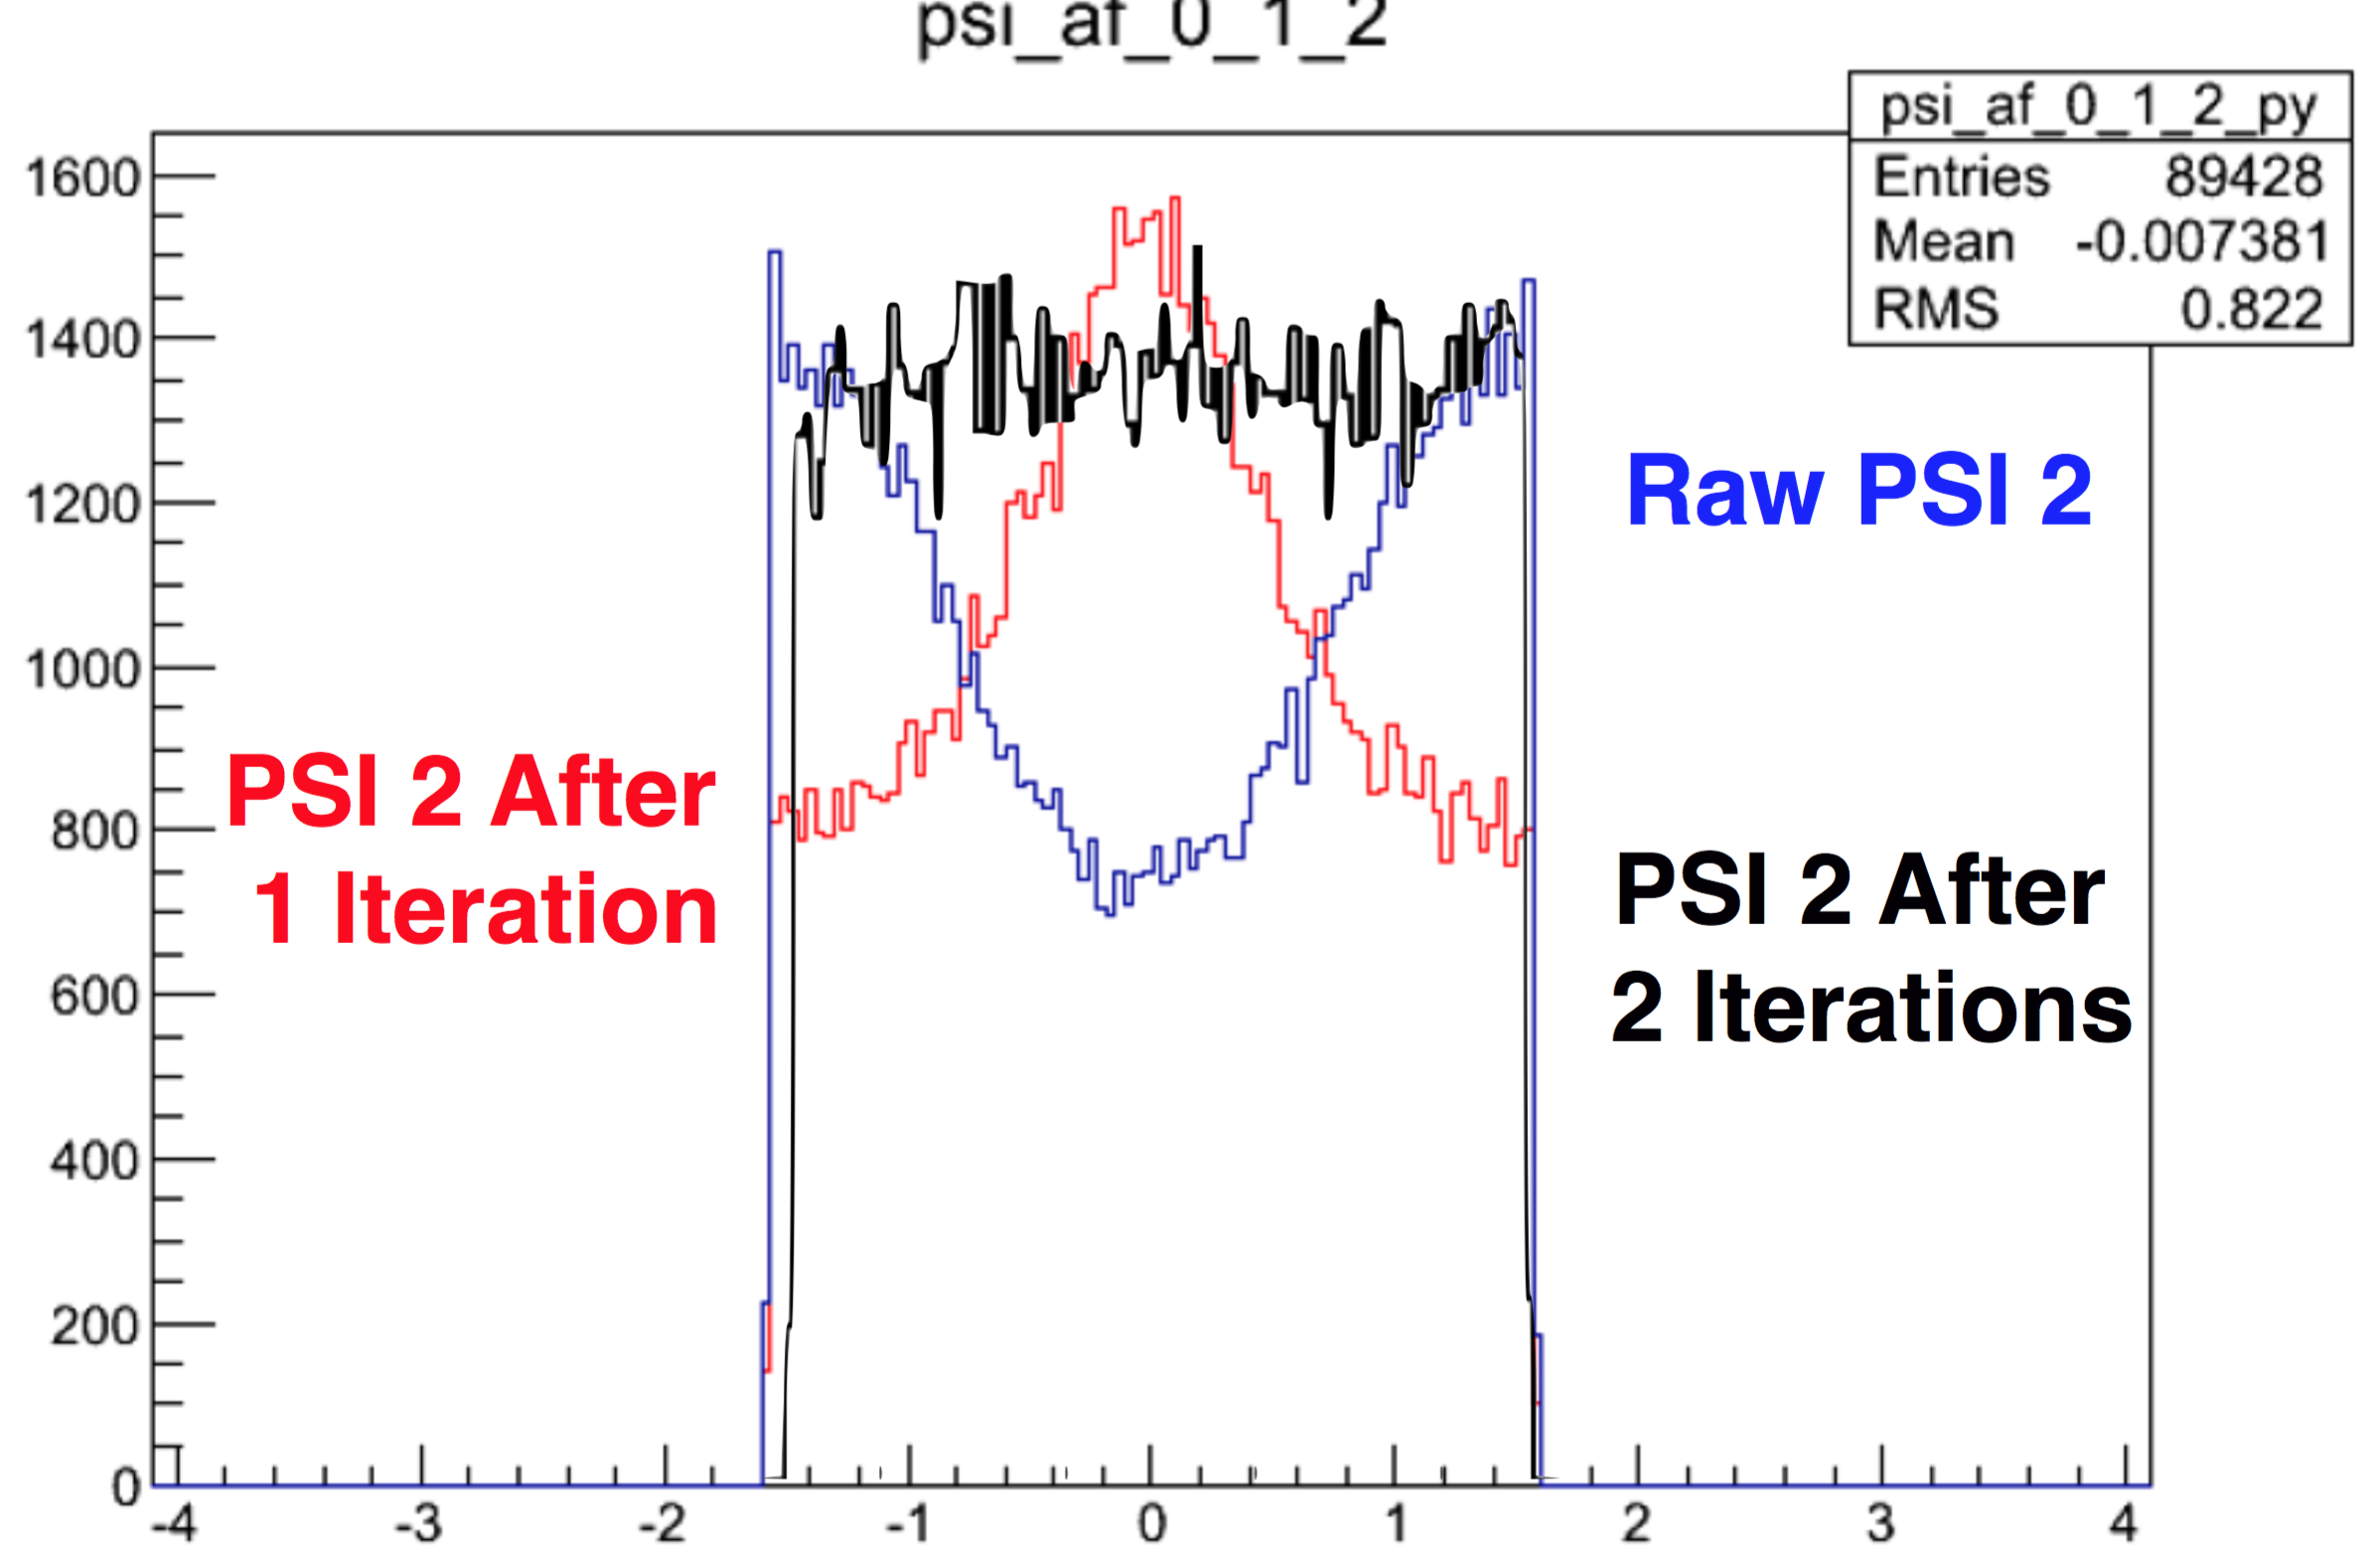
\includegraphics[width=0.65\linewidth]{figs/flatten_calib_iteration.png}
\caption{TBA}
\end{center}
\end{figure}
\begin{figure}[!h]
\begin{center}
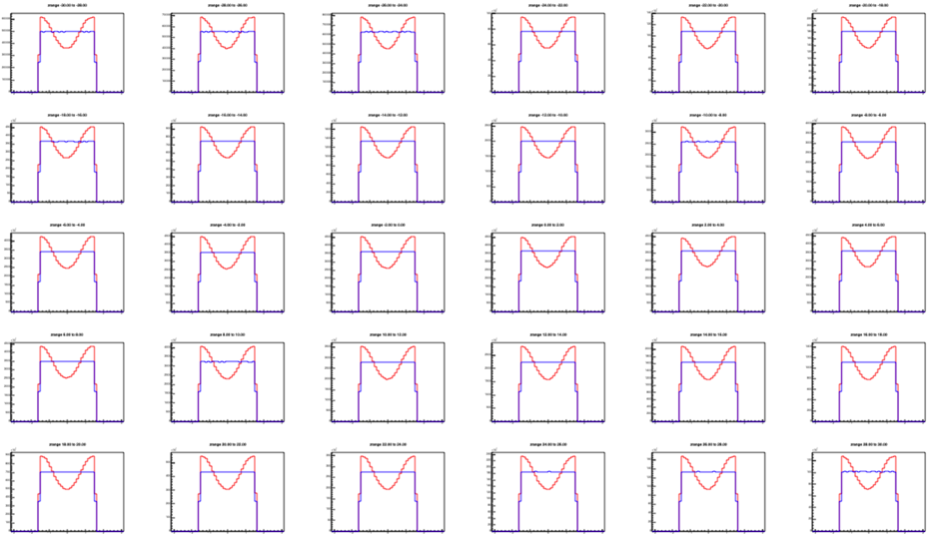
\includegraphics[width=0.65\linewidth]{figs/bbc_ep_bf_af.png}
\caption{BBC Psi2 EP distribution in different z vertex bins red before flattening, blue after flattening.}
\end{center}
\end{figure}
\subsection{Correcting for Beam Geometry}
\begin{figure}[!h]
\begin{center}
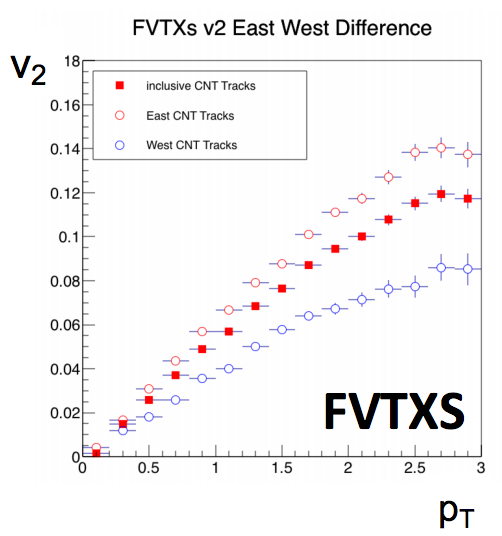
\includegraphics[width=0.4\linewidth]{figs/fvtx_ew_diff_bf.png}
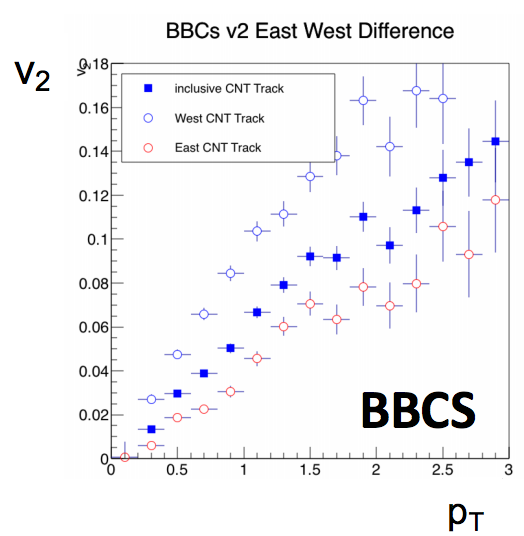
\includegraphics[width=0.4\linewidth]{figs/bbc_ew_diff_bf.png}
\caption{The left plot shows the FVTX EP East West Difference without any corrections and the right plot shows the BBC EP East West Difference without any corrections.}
\end{center}
\end{figure}
\begin{figure}[!h]
\begin{center}
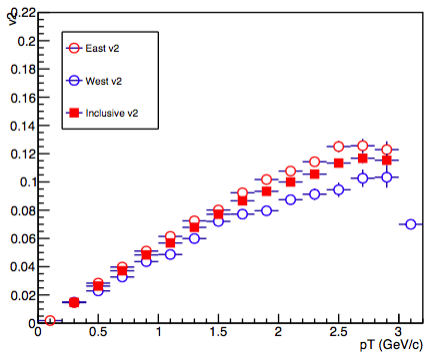
\includegraphics[width=0.4\linewidth]{figs/fvtx_rot_vtx.png}
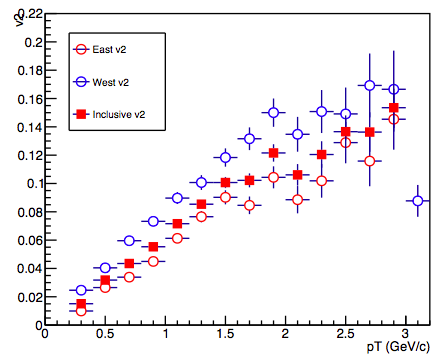
\includegraphics[width=0.4\linewidth]{figs/bbc_rot_vtx.png}
\caption{The left plot shows the FVTX EP East West Difference with beam rotation and vertex offset corrections and the right plot shows the BBC EP East West Difference with the same corrections.}
\end{center}
\end{figure}
\begin{figure}[!h]
\begin{center}
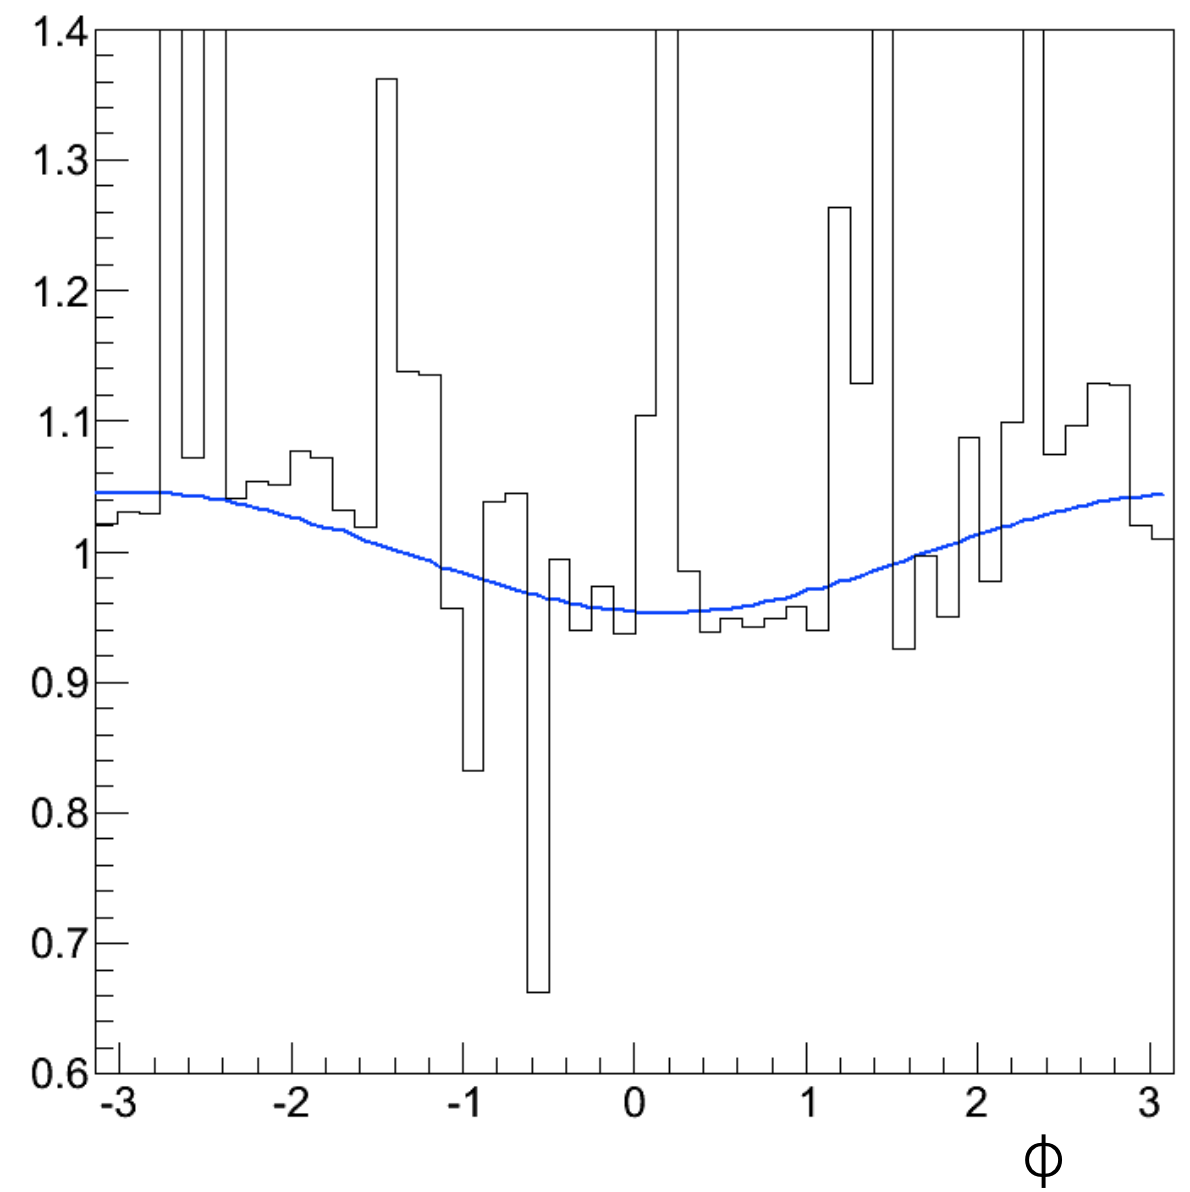
\includegraphics[width=0.5\linewidth]{figs/comparison_of_weights.png}
\caption{TBA}
\end{center}
\end{figure}
\begin{figure}[!h]
\begin{center}
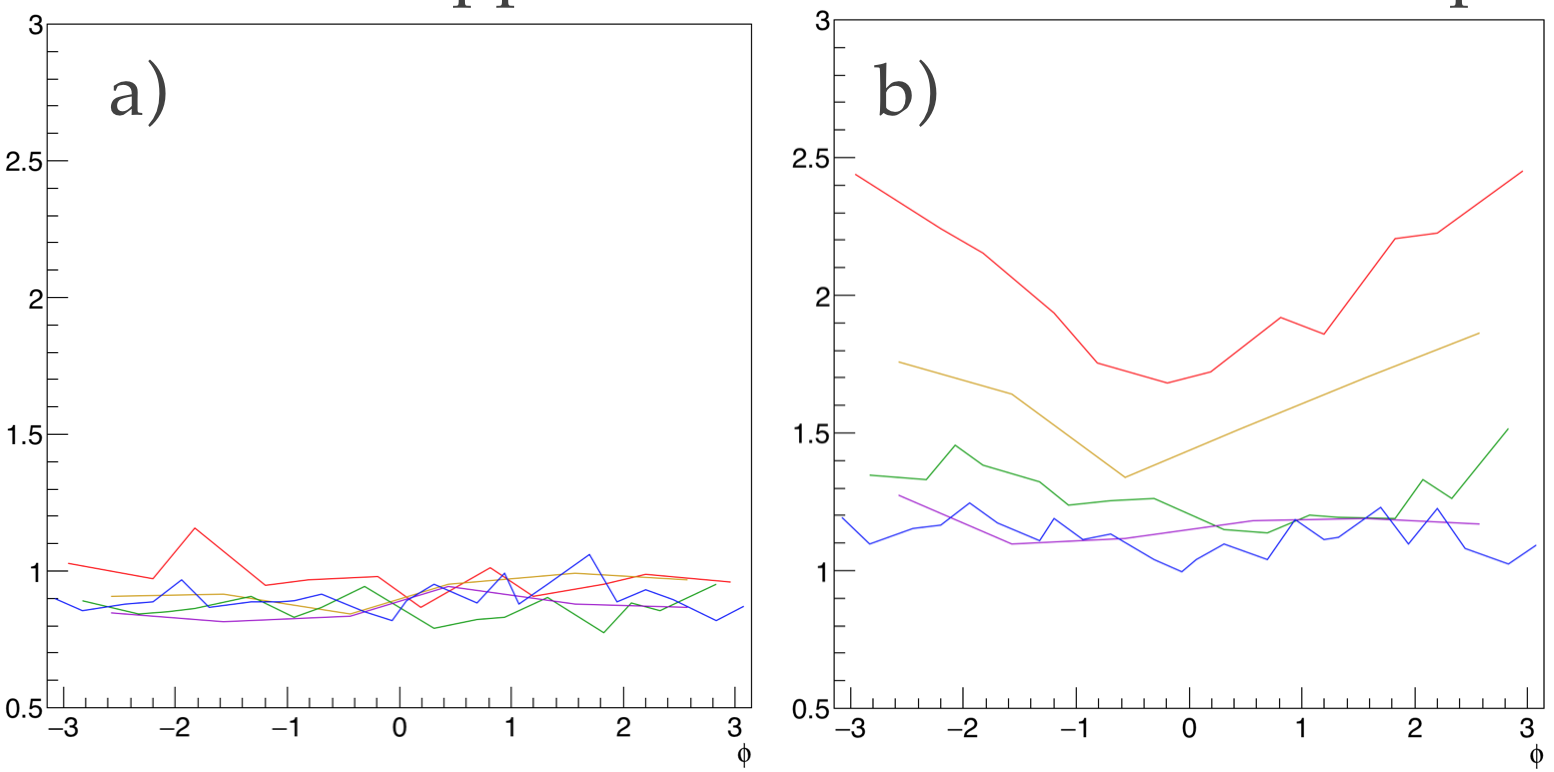
\includegraphics[width=0.6\linewidth]{figs/pp_pau_bbc_comparison.png}
\caption{These figures show the phi distribution of BBC PMT charge in a) the Run15 pp dataset and in b) the Run15 pAu dataset.}
\end{center}
\end{figure}
\begin{figure}[!h]
\begin{center}
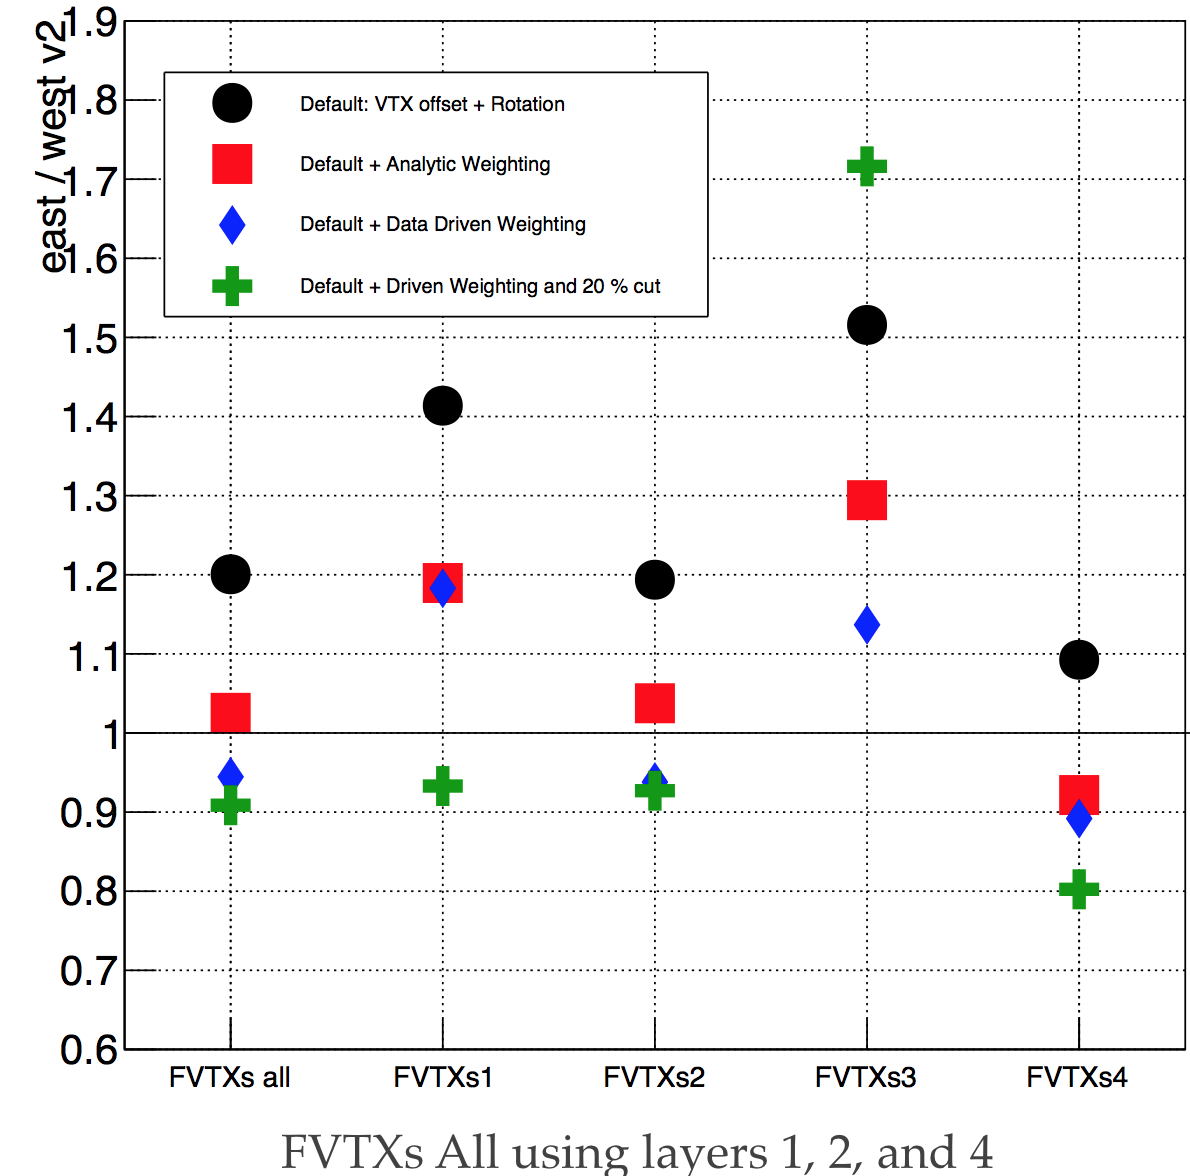
\includegraphics[width=0.5\linewidth]{figs/fvtx_correction_summary.png}
\caption{TBA}
\end{center}
\end{figure}
\begin{figure}[!h]
\begin{center}
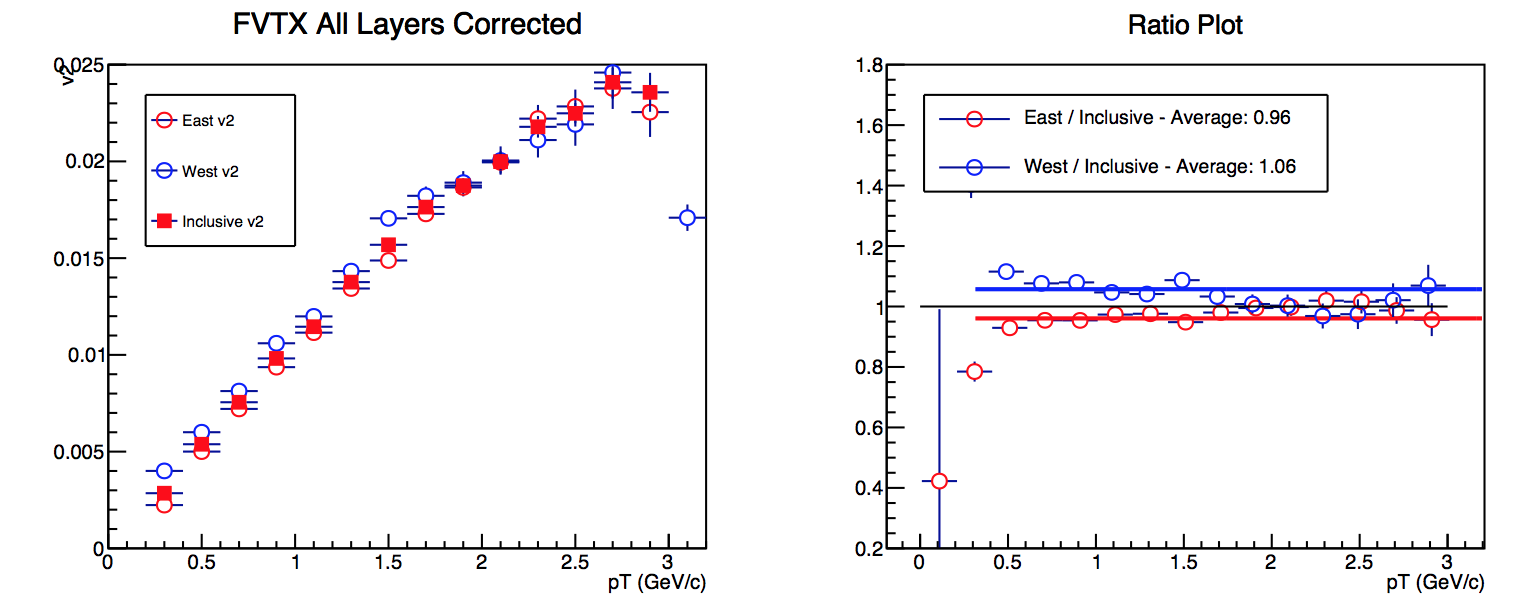
\includegraphics[width=0.5\linewidth]{figs/fvtx_corrected.png}
\caption{FVTX EP corrected with inverse $\phi$ weighting and 20 $\%$ cut.}
\end{center}
\end{figure}
\begin{figure}[!h]
\begin{center}
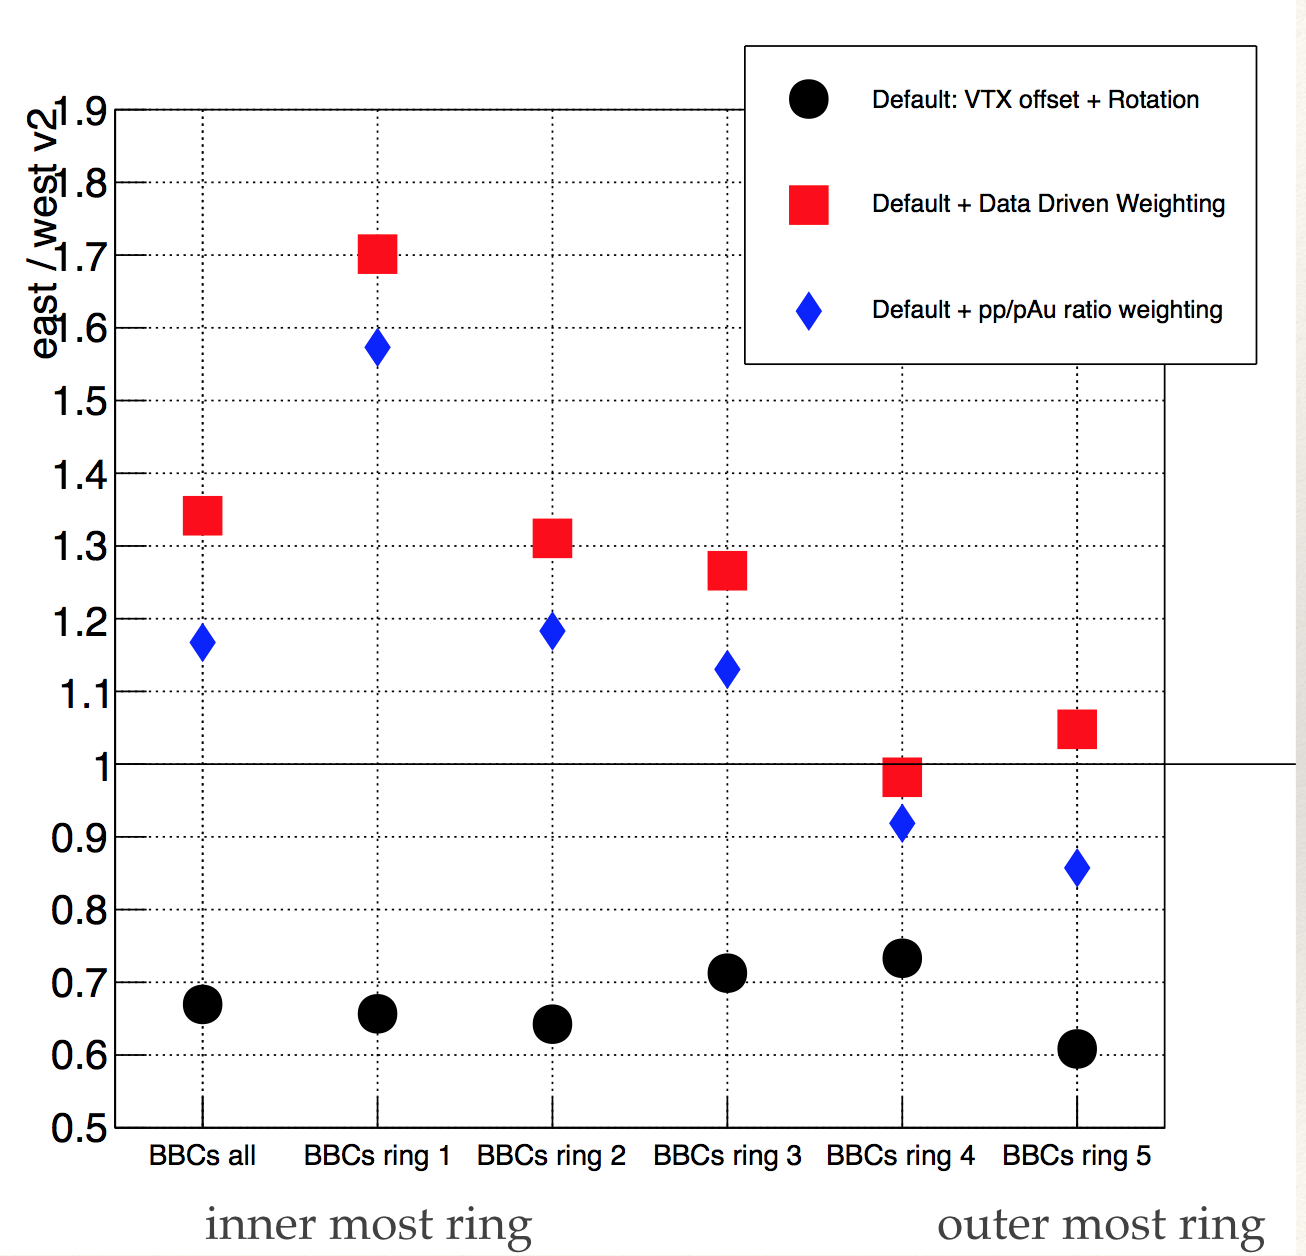
\includegraphics[width=0.5\linewidth]{figs/bbc_correction_summary.png}
\caption{TBA}
\end{center}
\end{figure}
\begin{figure}[!h]
\begin{center}
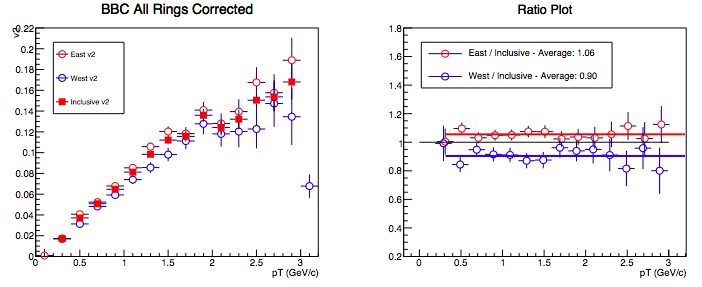
\includegraphics[width=0.5\linewidth]{figs/bbc_pp_correction.png}
\caption{BBC EP corrected with pp, pau ratio weighting.}
\end{center}
\end{figure}
\begin{figure}[!h]
\begin{center}
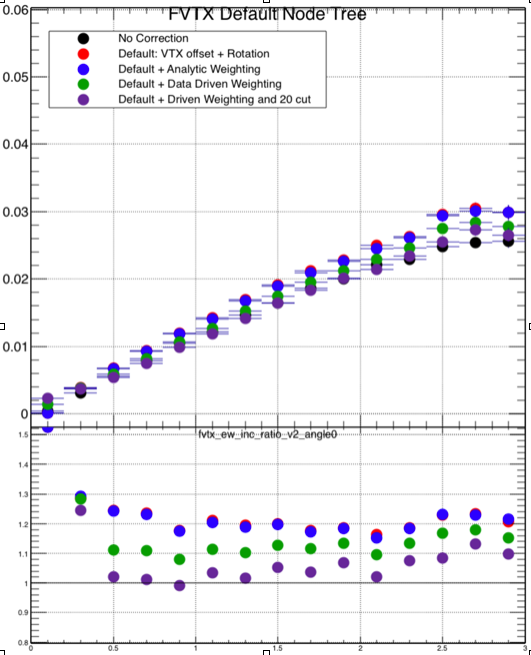
\includegraphics[width=0.5\linewidth]{figs/fvtx_incl_v2_comparison_corrections.png}
\caption{A comparison of FVTX EP $v_2$ corrections on the inclusive measurement.}
\end{center}
\end{figure}
\section{Systematic Error Estimate}
\subsection{Non-flow Estimate}
\begin{figure}[!h]
\begin{center}
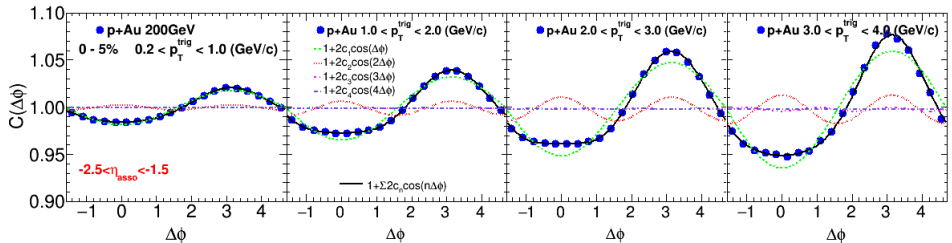
\includegraphics[width=0.6\linewidth]{figs/pau_correlation_central_fvtx.png}
\caption{TBA}
\end{center}
\end{figure}
\begin{figure}[!h]
\begin{center}
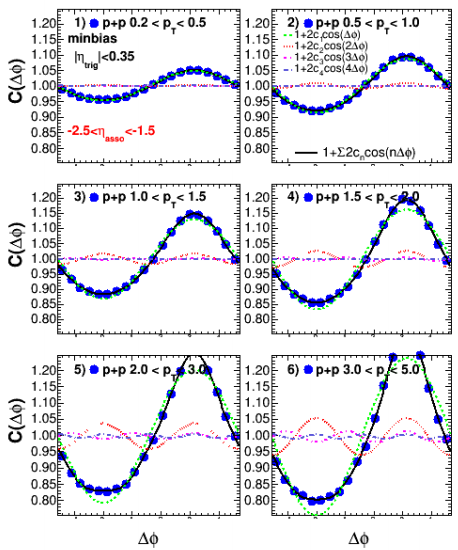
\includegraphics[width=0.6\linewidth]{figs/pp_correlation_minbias_fvtx.png}
\caption{TBA}
\end{center}
\end{figure}
\begin{figure}[!h]
\begin{center}
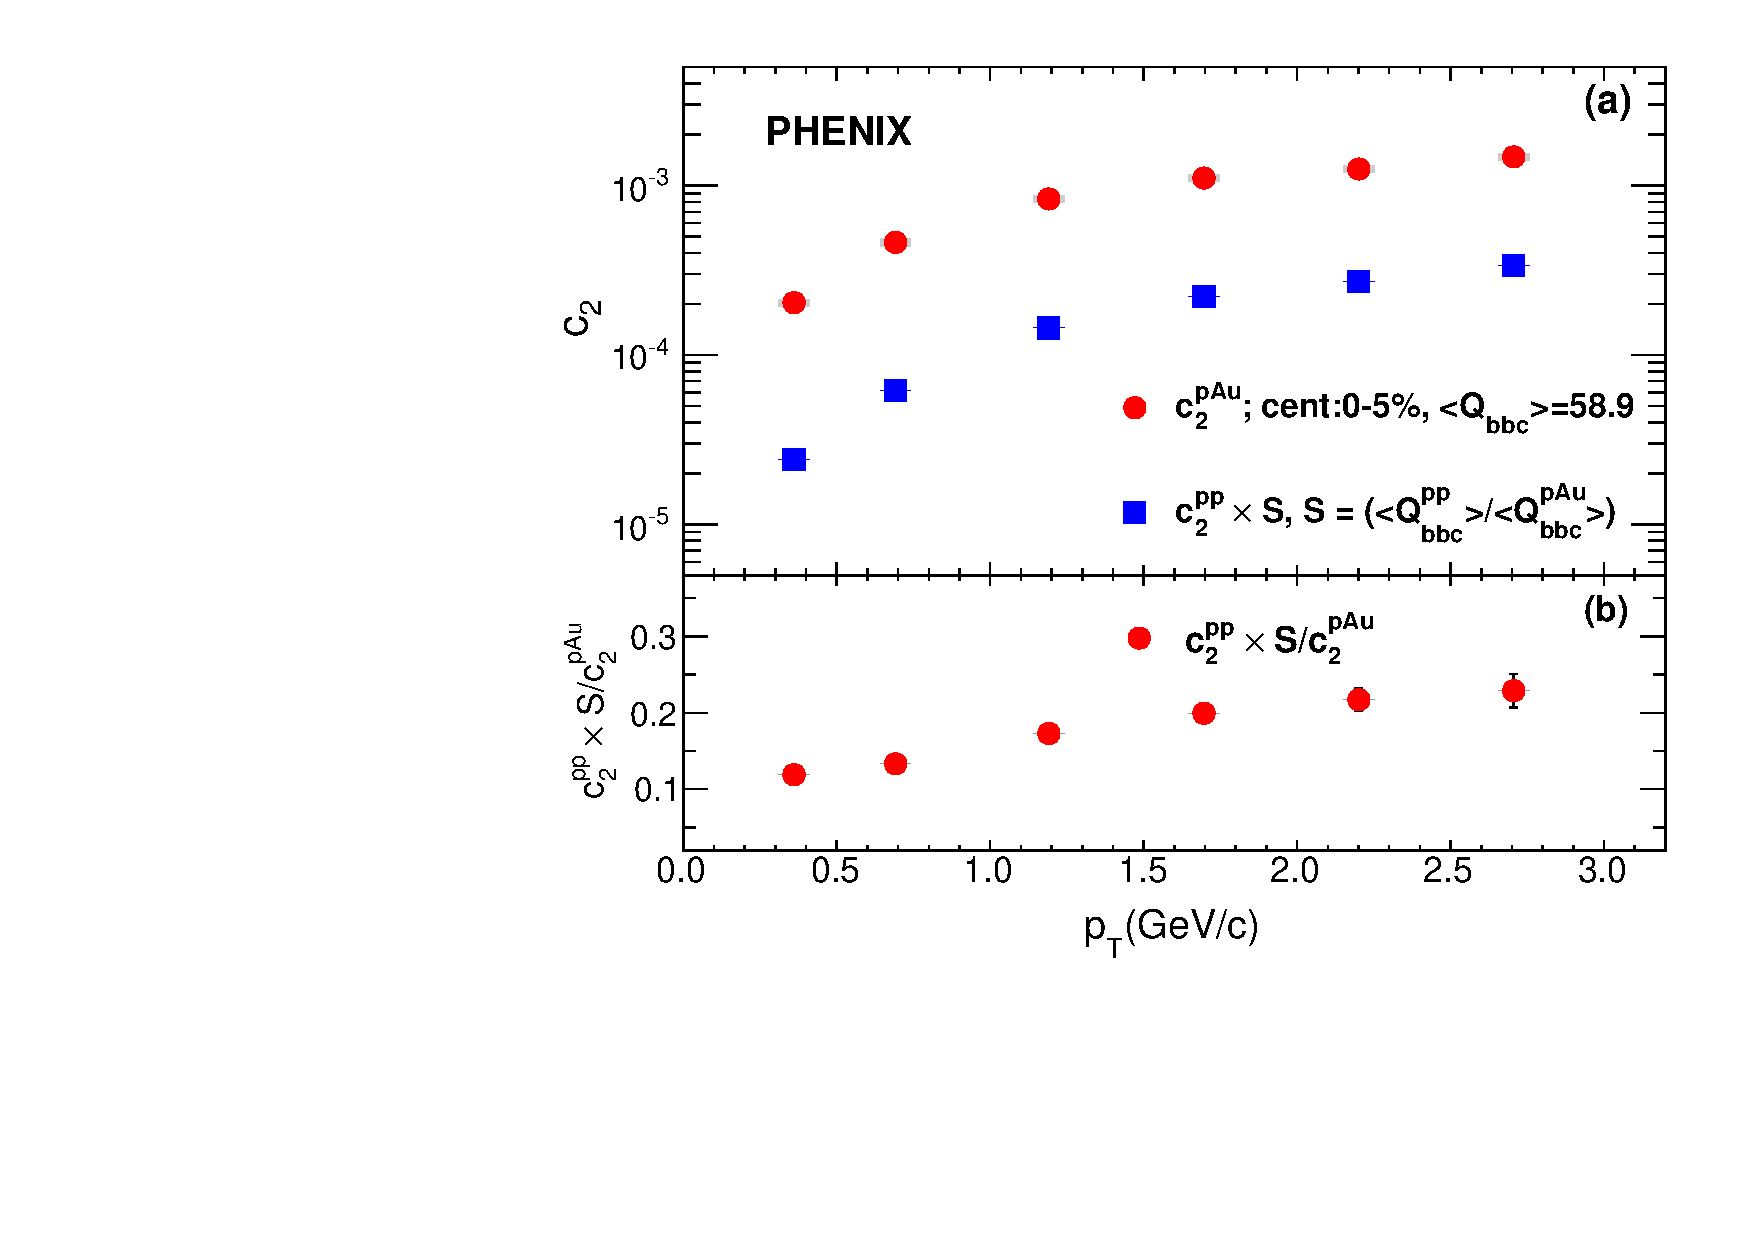
\includegraphics[width=0.6\linewidth]{figs/non_flow.pdf}
\caption{TBA}
\end{center}
\end{figure}
\subsection{Pile Up}
\begin{figure}[!h]
\begin{center}
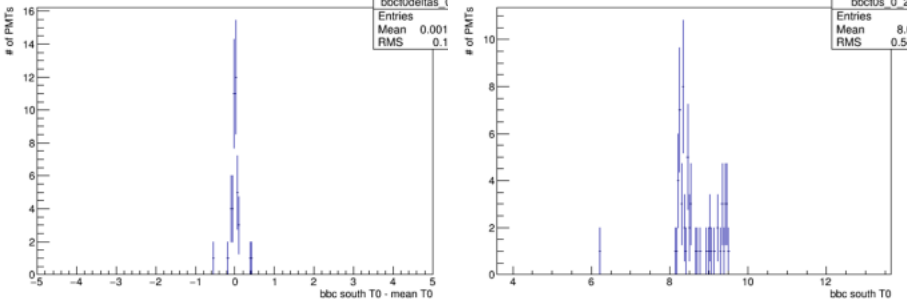
\includegraphics[width=0.6\linewidth]{figs/example_pile_up_event.png}
\caption{The left plot is an example of a normal event, the right plot is an example pile up event.}
\end{center}
\end{figure}
\subsection{Beam Angle}
\subsection{Track Background}
\subsection{Event Plane Detectors Agreement}
